\section{Results Discussion}

\subsection{Training}

% Arguments:

From Figure~\ref{fig:q-values} we can see the different performances from the 4 configuration. In order to reduce the noise of the Q-value estimates, as the cited papers did, during the training we take the averages of the Q-values from 64 steps, defined as \textit{epoch}. More epochs computed by a configuration implies more steps per episode and then more reward in general. Hence the \textit{deep} configurations played better than the \textit{shallow}. More details in the evaluation subsection.

A more interesting viewpoint is the overestimation issue. If the reward is nonzero and $\gamma < 1$ as in the \textit{CartPole} environment the return $G_t$ is $\frac{1}{1 - \gamma}$ \cite{Sutton:1998:IRL:551283}. Hence in our case the return with $\gamma = 0.99$ is $100$ then the DQN has to converge to that value.

From Figure~\ref{fig:q-values} we can see that the trends of all the configuration is to converge to 100. As described by \citeauthor{Hasselt:2016:DRL:3016100.3016191} \shortcite{Hasselt:2016:DRL:3016100.3016191} the Double Q-learning reduces the overestimation, in particular for the \textit{Double DQN deep} configuration, the \textit{DQN deep} suffers definitely of overestimation. For \textit{DQN shallow} configurations instead the differences are small, maybe the differences could start in later epochs.

\begin{figure*}[t]
	\centering
	\subfloat{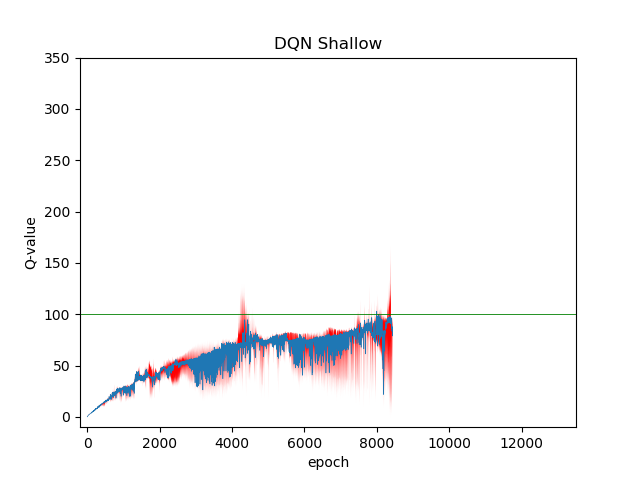
\includegraphics[width=.48\textwidth]{res/DQN_Shallow}} \quad
	\subfloat{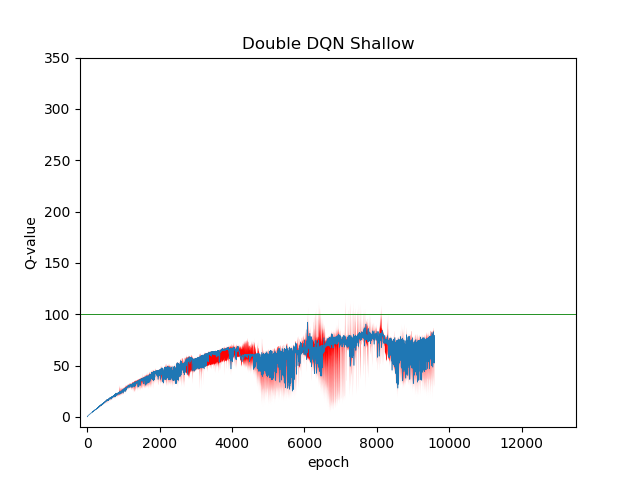
\includegraphics[width=.48\textwidth]{res/DoubleDQN_Shallow}} \\
	\subfloat{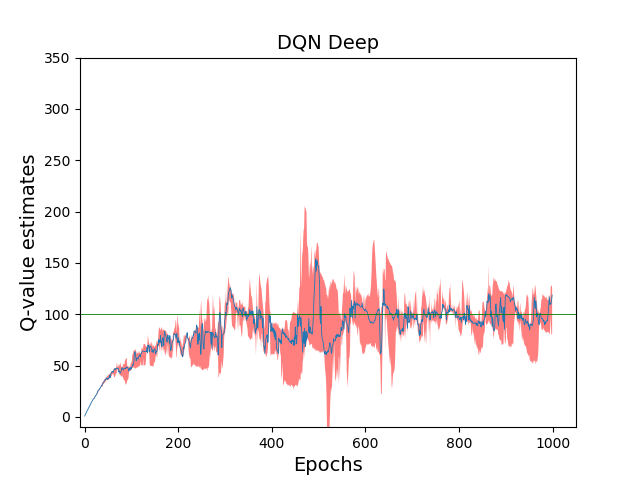
\includegraphics[width=.48\textwidth]{res/DQN_Deep}} \quad
	\subfloat{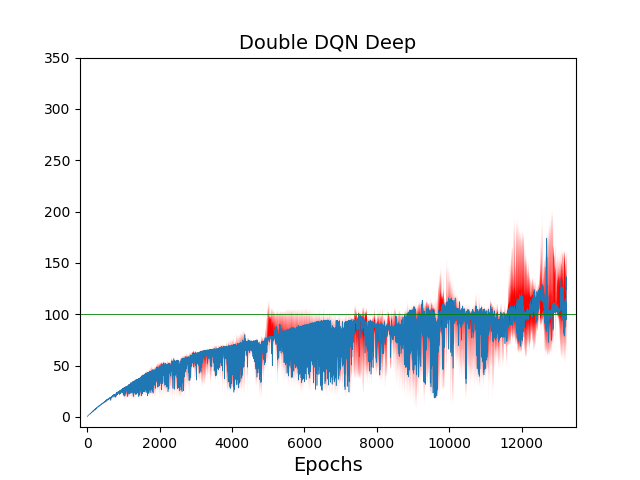
\includegraphics[width=.48\textwidth]{res/DoubleDQN_Deep}} \\
	
	%\subfloat[][\emph{Cascata}.]
	%{\includegraphics[width=.45\textwidth]{Cascata}} \quad
	%\subfloat[][\emph{Salita e discesa}.]
	%{\includegraphics[width=.45\textwidth]{SalitaDiscesa}}
	\caption{The plots shows the Q-value estimates performance for each configuration running for 3600 episodes. Each episode performs every step depending on the good or bad interaction of the agent. This means that some agent finished in less steps. Each point on the blue lines is the median Q-value per epoch (the average Q-value computed every 64 steps) of 3 executions with different seed. The red area shows the maximum and minimum Q-value per epoch of 3 executions with different seed.}
	\label{fig:q-values}
\end{figure*}


\subsection{Evaluation}

% Theses:
From the results of evaluation (Figure~\ref{fig:comparison}) of the model we can see that our \textit{DQN deep} is better for all the seeds. The model after 1000 episodes of learning is able to \textit{solve} the \textit{CartPole} problem. It is a good result considering that we not tuned the algorithm hyperparameters.

A further interesting fact that emerges from the Figure~\ref{fig:comparison} is that a different seed could imply a good or a bad learning process. The \textit{DQN shallow} configuration showed that for the best seed needs 1300 episode in order to solve the problem while the seed 52 needs 2000 episode.

\begin{figure}
	\centering
	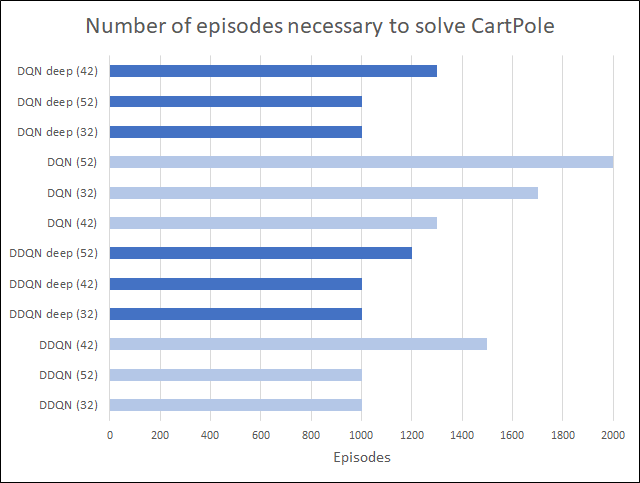
\includegraphics[width=0.48\textwidth]{res/Comparison}
	\caption{text}
	\label{fig:comparison}
\end{figure}
